% Generator: hand-authored TikZ schematic.
% Source ID: src-1c1b7702523f8dab3f1fb274ae6d8c631a291090d33ddb6e3d9f3d8de897a1d0
% PDF SHA-256: 88b72fea05d331215504bb89257e375d07c18ba21e830cf9e6288461e88ccf8d
% Source location: PDF page 1, printed page 138, Question 18.
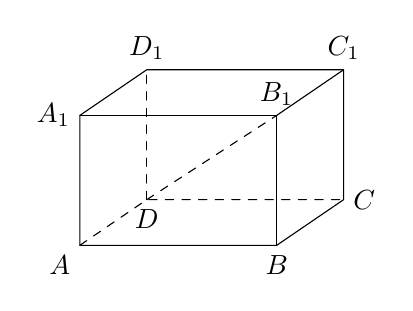
\begin{tikzpicture}[line cap=round,line join=round]
  % Schematic projection only; edge lengths and angles are not asserted.
  \coordinate (A)  at (0,0);
  \coordinate (B)  at (2.5,0);
  \coordinate (C)  at (3.35,0.58);
  \coordinate (D)  at (0.85,0.58);
  \coordinate (A1) at (0,1.65);
  \coordinate (B1) at (2.5,1.65);
  \coordinate (C1) at (3.35,2.23);
  \coordinate (D1) at (0.85,2.23);

  % Solid visible edges.
  \draw (A)--(B)--(C)--(C1)--(D1)--(A1)--(A);
  \draw (A1)--(B1)--(B);
  \draw (B1)--(C1);
  % Hidden edges and the explicitly shown diagonal B1D.
  \draw[dashed] (A)--(D)--(C);
  \draw[dashed] (D)--(D1);
  \draw[dashed] (D)--(B1);

  \node[below left] at (A) {$A$};
  \node[below] at (B) {$B$};
  \node[right] at (C) {$C$};
  \node[below] at (D) {$D$};
  \node[left] at (A1) {$A_1$};
  \node[above] at (B1) {$B_1$};
  \node[above] at (C1) {$C_1$};
  \node[above] at (D1) {$D_1$};
\end{tikzpicture}
